\documentclass[conference]{IEEEtran}
\usepackage{amsmath,amssymb}
\usepackage{graphicx}
\usepackage{booktabs}
\usepackage{longtable}
\usepackage{array}
\usepackage{url}
\usepackage{cite}
\usepackage[hidelinks]{hyperref}
\usepackage{microtype}
\setlength{\emergencystretch}{1.5em}
\providecommand{\tightlist}{\setlength{\itemsep}{0pt}\setlength{\parskip}{0pt}}
\title{AI-Driven Hostel Food Waste Mitigation and Demand Forecasting
System: A Reproducible Machine-Learning Framework for Institutional
Dining}
\author{\IEEEauthorblockN{Author Name(s)}\\
\IEEEauthorblockA{Department / Institution\\City, Country\\email@example.com}}
\begin{document}
\maketitle
\begin{abstract}
Institutional hostels must prepare meals before exact student participation is known, creating a recurring trade-off between service availability and avoidable food waste. This paper presents an AI-driven demand-forecasting and preparation-recommendation framework for hostel dining operations. The system is designed as a reproducible engineering pipeline comprising: (i) a synthetic meal-level data generator for controlled experimentation; (ii) leakage-aware preprocessing and chronological train-test evaluation; (iii) Linear Regression, Random Forest, and XGBoost regression models for student-turnout forecasting; and (iv) an operational policy that converts forecast attendance into recommended preparation weight using meal-specific per-student consumption and a configurable safety buffer. The default synthetic dataset contains 2,193 breakfast, lunch, and dinner observations spanning two years, with explanatory variables representing hostel occupancy, advance bookings, menu popularity, examinations, weekends, vacations, special events, temperature, and rainfall intensity. On a chronological holdout of 441 observations, Linear Regression achieved MAE 10.158 students, RMSE 12.825 students, and R² 0.9736; XGBoost achieved MAE 10.345 students with RMSE 13.152 and R² 0.9722, while Random Forest achieved MAE 10.565, RMSE 13.521, and R² 0.9706. A retrospective operational simulation with a 3% buffer reduced modeled leftover food from 8,423.00 kg to 2,600.69 kg while introducing simulated shortage equivalent to 1.077% of realized consumption. These results demonstrate the engineering feasibility of coupling demand prediction with an explicit preparation decision rule. Because the experiments use synthetic data, the reported savings are simulation outcomes and require validation on real hostel records before institutional or causal claims are made.
\end{abstract}
\begin{IEEEkeywords}
food waste, demand forecasting, hostel dining, institutional catering, machine learning, Random Forest, XGBoost, sustainability, decision support.
\end{IEEEkeywords}

\subsection{Introduction}\label{introduction}

Food waste is a sustainability, cost, and resource-allocation problem
across households, retail, and food-service systems. The United Nations
Sustainable Development Goal (SDG) 12.3 calls for halving per-capita
global food waste at retail and consumer levels by 2030 {[}1{]}. The
United Nations Environment Programme (UNEP) Food Waste Index Report 2024
further emphasizes the need for systematic measurement and practical
waste-reduction interventions across food-service settings {[}2{]}. For
institutional kitchens, one particularly actionable intervention is to
improve the decision made before a meal is prepared: \textbf{how many
people are likely to eat, and how much food should be produced?}

Hostel dining is a useful engineering context because meal demand is
recurrent yet non-stationary. Student participation varies by breakfast,
lunch, and dinner; by weekday and weekend; during examinations and
vacations; with menu popularity; and in response to temporary events.
Kitchen staff commonly compensate for this uncertainty by preparing a
safety surplus. The surplus protects service quality but increases
leftover food if the estimated turnout is too high. Conversely,
aggressive reductions in preparation may create shortages and reduce
service reliability. A deployable system therefore should not optimize
forecast accuracy in isolation. It should connect prediction to a
transparent operational policy that exposes the waste-versus-shortage
trade-off.

Prior work supports the relevance of data-driven forecasting in
catering. Rodrigues \emph{et al.} evaluated machine-learning demand
forecasting across catering services and reported that improved
forecasting could reduce wasted meals while also reducing unmet demand
relative to baseline approaches {[}3{]}. Faezirad \emph{et al.} modeled
university dining attendance and reservation behavior for food-waste
prevention {[}4{]}. Recent campus-focused work has applied regression
models including XGBoost for meal-demand estimation {[}5{]}, while Aydın
\emph{et al.} compared XGBoost, LSTM, and Prophet for institutional
cafeteria forecasting {[}6{]}. Public catering research by Malefors
\emph{et al.} has similarly shown that machine-learning attendance
forecasts can create economic and waste-reduction opportunities,
particularly when demand patterns are disrupted {[}7{]}.

Despite this progress, three practical gaps frequently arise in student
capstone implementations. First, many demonstrations use random
train-test splits even when the deployment problem is temporal
forecasting, which can yield optimistic estimates. Second, target
leakage may occur if variables available only after food
preparation---such as actual food prepared, actual waste, or realized
attendance-derived quantities---are included among predictive features.
Third, a model may predict attendance without specifying how that
prediction should influence the final kitchen decision. Forecasting
alone does not determine a preparation quantity unless a consumption
model and service-level buffer are defined.

This work addresses these gaps through a deliberately modular
engineering architecture. The forecasting layer is restricted to
pre-meal information. Data are split chronologically so that the model
is evaluated on later dates than those used for training. The
operational layer then estimates a robust meal-specific consumption rate
in kilograms per attending student and applies a configurable safety
margin. The resulting system produces two outputs useful to a kitchen
manager: expected turnout and recommended preparation mass.

The contributions of this paper are as follows:

\begin{enumerate}
\def\labelenumi{\arabic{enumi}.}
\tightlist
\item
  A reproducible synthetic dataset generator producing more than 1,500
  meal-level observations with realistic operational, academic, menu,
  and environmental factors.
\item
  A leakage-aware forecasting pipeline comparing a linear baseline with
  Random Forest and XGBoost ensemble regressors using MAE, RMSE, and R².
\item
  A mathematically explicit food-preparation policy linking predicted
  turnout to kilograms of food while separately measuring simulated
  leftovers and shortages.
\item
  A chronological evaluation design and complete GitHub-ready
  implementation supporting reproducibility, testing, model
  serialization, and single-meal inference.
\item
  A transparent research-integrity boundary: all reported experimental
  results are identified as synthetic simulation results rather than
  empirical hostel measurements.
\end{enumerate}

The remainder of the paper reviews related work, formalizes the
prediction and decision problem, presents the architecture and dataset
design, reports experimental results, and discusses deployment
implications and limitations.

\subsection{Related Work}\label{related-work}

\subsubsection{Food Waste in Institutional and Food-Service
Systems}\label{food-waste-in-institutional-and-food-service-systems}

Food-service waste is influenced by planning, customer behavior, menu
design, serving practices, and the mismatch between production and
realized consumption. Dhir \emph{et al.} reviewed food waste in
hospitality and food services and organized prior research around
generation drivers, waste-reduction practices, stakeholder behavior, and
leftover handling {[}8{]}. Such evidence motivates upstream
interventions that prevent excess production rather than dealing only
with food after it becomes waste.

UNEP's Food Waste Index work provides a global measurement context and
emphasizes systematic measurement across food-service and other
consumer-facing sectors {[}2{]}. At the operational scale, institutional
dining creates an especially measurable setting because demand can be
observed repeatedly at scheduled meals, and explanatory variables such
as bookings, academic calendars, menu plans, and occupancy are often
available in structured information systems.

\subsubsection{Demand Forecasting for Catering and
Canteens}\label{demand-forecasting-for-catering-and-canteens}

Rodrigues \emph{et al.} compared machine-learning forecasting methods
using real catering-service datasets covering multiple years. Their
results showed that Random Forest and LSTM models could improve demand
estimates and that better predictions could translate into lower waste
and unmet demand {[}3{]}. Their study is particularly relevant because
it evaluates the downstream operational consequences of forecasts rather
than treating forecasting metrics as the only objective.

Posch \emph{et al.} developed a Bayesian approach for food and beverage
sales prediction in staff canteens and restaurants, highlighting the
role of accurate forecasting in purchasing and pre-consumer waste
reduction {[}9{]}. Public catering research by Eriksson and colleagues
also demonstrated the potential value of machine-learning attendance
prediction under the distributional disruption associated with the
COVID-19 period {[}7{]}. These studies support a broader conclusion:
food-service demand contains structured patterns but can be affected by
calendar changes, behavior, and exogenous events.

In university dining, Faezirad \emph{et al.} explicitly modeled
reservations and show/no-show behavior and used an
artificial-neural-network-aided formulation to support waste prevention
{[}4{]}. Turker examined campus dining demand using multiple
machine-learning regressors, including XGBoost, and emphasized links
among campus density, food preferences, and required meal counts
{[}5{]}. Aydın \emph{et al.} compared XGBoost, LSTM, and Prophet in an
institutional demand-forecasting case, showing that different methods
may perform differently depending on temporal resolution and forecasting
horizon {[}6{]}.

\subsubsection{Machine Learning for Food-Waste Monitoring and
Prediction}\label{machine-learning-for-food-waste-monitoring-and-prediction}

Machine learning is also being used beyond demand forecasting. Li
\emph{et al.} proposed a machine-vision recognition approach to identify
food waste in university cafeterias {[}10{]}. More recent work has
examined direct prediction of waste quantity in large-scale dining
facilities {[}11{]}. These directions are complementary to the current
work. Vision and weighing systems can quantify what was wasted after
service, whereas demand forecasting aims to prevent a portion of that
waste before production.

From a modeling perspective, Random Forest is a robust bagging ensemble
that averages decorrelated decision trees and can capture nonlinearities
and interactions without requiring strong parametric assumptions
{[}12{]}. XGBoost is a gradient-boosted decision-tree framework designed
for regularized, scalable learning and has become common in tabular
prediction tasks {[}13{]}. These models are appropriate candidates for
meal-demand forecasting because attendance may depend nonlinearly on
occupancy, bookings, meal type, calendar state, weather, and menu
characteristics.

\subsubsection{Research Gap and
Positioning}\label{research-gap-and-positioning}

Existing work establishes the value of demand forecasting, but an
engineering capstone still needs careful separation between four
concepts: \textbf{inputs available before a meal}, \textbf{forecast
target}, \textbf{consumption conversion}, and \textbf{operational
decision rule}. The present framework makes those boundaries explicit.
Actual prepared kilograms and actual waste are excluded from
turnout-model features because they are post-decision variables. The
model predicts attendance first. A second layer then converts attendance
to preparation mass. This modularity improves interpretability, supports
service-level tuning, and reduces the risk that a high evaluation score
is caused by leakage.

A further distinction is the use of a synthetic generator as a
development instrument. Synthetic data allow the software, validation
rules, modeling pipeline, and reproducibility mechanisms to be tested
before sensitive institutional records are available. However, synthetic
experiments cannot establish field effectiveness. Accordingly, this
study positions its results as an engineering demonstration and defines
real-world validation as a required next phase.

\subsection{Problem Definition and Mathematical
Formulation}\label{problem-definition-and-mathematical-formulation}

Let each observation correspond to date \(t\) and meal category
\(m\in\{B,L,D\}\), representing breakfast, lunch, and dinner. Define the
pre-meal feature vector

\[
\mathbf{x}_{t,m} = [\mathbf{c}_t,\mathbf{h}_t,\mathbf{a}_t,\mathbf{u}_{t,m},\mathbf{e}_t],
\]

where \(\mathbf{c}_t\) contains calendar variables, \(\mathbf{h}_t\)
hostel occupancy and booking variables, \(\mathbf{a}_t\) academic-status
variables such as examinations and vacations, \(\mathbf{u}_{t,m}\) meal
and menu variables, and \(\mathbf{e}_t\) environmental variables.

The first-stage supervised-learning problem is

\[
\hat{N}_{t,m}=f_{\theta}(\mathbf{x}_{t,m}),
\]

where \(N_{t,m}\) is realized student turnout and \(f_{\theta}\) is a
fitted regression model. Three model classes are evaluated: Linear
Regression, Random Forest Regression, and XGBoost Regression.

Forecast accuracy is measured using Mean Absolute Error (MAE), Root Mean
Squared Error (RMSE), and coefficient of determination \(R^2\):

\[
\mathrm{MAE}=\frac{1}{n}\sum_{i=1}^{n}|N_i-\hat{N}_i|,
\]

\[
\mathrm{RMSE}=\sqrt{\frac{1}{n}\sum_{i=1}^{n}(N_i-\hat{N}_i)^2},
\]

\[
R^2=1-\frac{\sum_i(N_i-\hat{N}_i)^2}{\sum_i(N_i-\bar{N})^2}.
\]

The second stage converts predicted attendance into a preparation
recommendation. For each meal category \(m\), let \(q_m\) be the median
kilograms consumed per attending student estimated \textbf{only from the
training partition}:

\[
q_m=\operatorname{median}_{(t,m)\in\mathcal{T}}
\left(\frac{C_{t,m}}{N_{t,m}}\right),
\]

where \(C_{t,m}\) is realized food consumption and \(\mathcal{T}\)
denotes training data. For safety buffer \(b\geq0\), recommended
preparation is

\[
\hat{P}_{t,m}=\hat{N}_{t,m}\,q_m(1+b).
\]

This policy is intentionally simple and auditable. The parameter \(b\)
captures the institution's service-level tolerance. A larger value
reduces shortage risk but increases potential leftovers.

For retrospective analysis, simulated leftover and shortage are defined
as

\[
L_{t,m}=\max(\hat{P}_{t,m}-C_{t,m},0),
\]

\[
S_{t,m}=\max(C_{t,m}-\hat{P}_{t,m},0).
\]

The operational goal is therefore multi-objective: minimize forecast
error and leftover food while constraining shortage to an acceptable
level. A future deployment can select \(b\) by solving

\[
\min_b \; \alpha\sum L_{t,m}+\beta\sum S_{t,m},
\]

where \(\alpha\) represents the cost of waste and \(\beta\) represents
the higher service penalty that may be assigned to shortages.

\subsection{Dataset and Synthetic Data
Generator}\label{dataset-and-synthetic-data-generator}

\subsubsection{Purpose of Synthetic
Data}\label{purpose-of-synthetic-data}

The dataset generator is included so that the complete engineering
pipeline can be executed without exposing student records or claiming
access to institutional measurements. The generator is deterministic
under a fixed random seed and contains explicit validation rules. It
should be replaced with audited operational data for a real study.

The default period is 1 January 2024 through 31 December 2025. Three
meal observations are generated per day, producing 2,193 records. Hostel
capacity is fixed at 520 in the default configuration, while the number
of residents physically present varies according to weekends,
examination periods, vacations, festival periods, and random day-to-day
variation.

\subsubsection{Variables}\label{variables}

The dataset includes the following groups.

\textbf{1) Calendar variables:} year, month, day of week, day name, and
weekend indicator.

\textbf{2) Academic variables:} examination, vacation, festival, and
special-event flags.

\textbf{3) Hostel variables:} hostel capacity, residents present, and
advance bookings.

\textbf{4) Meal variables:} breakfast/lunch/dinner category, menu name,
and menu-popularity score.

\textbf{5) Environmental variables:} temperature and normalized
rain-intensity index.

\textbf{6) Outcomes:} student turnout, average consumption per attending
student, food consumed, food prepared, food wasted, waste percentage,
and estimated waste cost.

The generator assigns different base turnout and portion-consumption
profiles to breakfast, lunch, and dinner. Menu popularity modifies
turnout, while examinations, weekends, events, rainfall, and temperature
introduce systematic and stochastic variation. Food preparation is
generated by applying conservative planning noise and a meal-specific
surplus to realized consumption, after which a small plate-waste
component is added.

\subsubsection{Validation}\label{validation}

Before a generated dataset is written, the software checks that (i) more
than 1,500 observations exist, (ii) no required values are missing,
(iii) attendance never exceeds residents present, (iv) waste is
nonnegative, and (v) prepared food is strictly positive. These checks
are important because a synthetic generator can otherwise silently
produce impossible records that inflate or destabilize downstream
models.

\subsection{Model Architecture and
Implementation}\label{model-architecture-and-implementation}

\subsubsection{Leakage-Aware Feature
Boundary}\label{leakage-aware-feature-boundary}

Only variables plausibly available before meal preparation are used to
predict turnout: calendar fields, residents present, advance bookings,
academic flags, temperature, rain index, meal category, menu name, and
menu-popularity score. The model excludes realized food consumption,
prepared food, and wasted food.

Categorical features are one-hot encoded with unknown-category handling.
Numeric variables are median-imputed and standardized. Although the
current synthetic dataset contains no missing values, keeping imputation
in the production pipeline protects deployment against incomplete
records.

\subsubsection{Chronological Evaluation}\label{chronological-evaluation}

A random row split would allow records from late dates to appear in the
training set while earlier dates appear in the test set. That is
inconsistent with the intended use case, where a trained model predicts
future meals. The implementation therefore sorts by date, identifies
unique dates, and assigns the earliest 80\% of dates to training and the
latest 20\% to testing. Whole dates are kept together so breakfast,
lunch, and dinner from the same date cannot be split across partitions.

The default run produced 1,752 training observations from 1 January 2024
to 6 August 2025 and 441 holdout observations from 7 August 2025 to 31
December 2025.

\subsubsection{Candidate Models}\label{candidate-models}

\textbf{Linear Regression} is used as a strong interpretable baseline
because much of institutional demand can be explained through additive
effects and bookings.

\textbf{Random Forest} uses 450 regression trees, bounded depth, minimum
leaf-size regularization, feature subsampling, and parallel fitting. It
is expected to capture nonlinear interactions, threshold behavior, and
heterogeneous effects without a manually specified functional form
{[}12{]}.

\textbf{XGBoost} uses histogram-based gradient-boosted trees with
shrinkage, row and column subsampling, L1/L2 regularization, and a
squared-error objective {[}13{]}. It is included because gradient
boosting frequently performs strongly on heterogeneous tabular data.

All models share the same chronological partitions and the same
permitted predictor set.

\subsubsection{Architecture}\label{architecture}

The system is organized as the following data flow:

The trained best model is serialized with Joblib. Model metadata store
the training/test ranges, selected model name, safety buffer,
meal-specific consumption coefficients, and aggregated operational
simulation. A separate inference script accepts JSON pre-meal features
and returns predicted turnout and recommended kilograms.

\begin{figure}
\centering
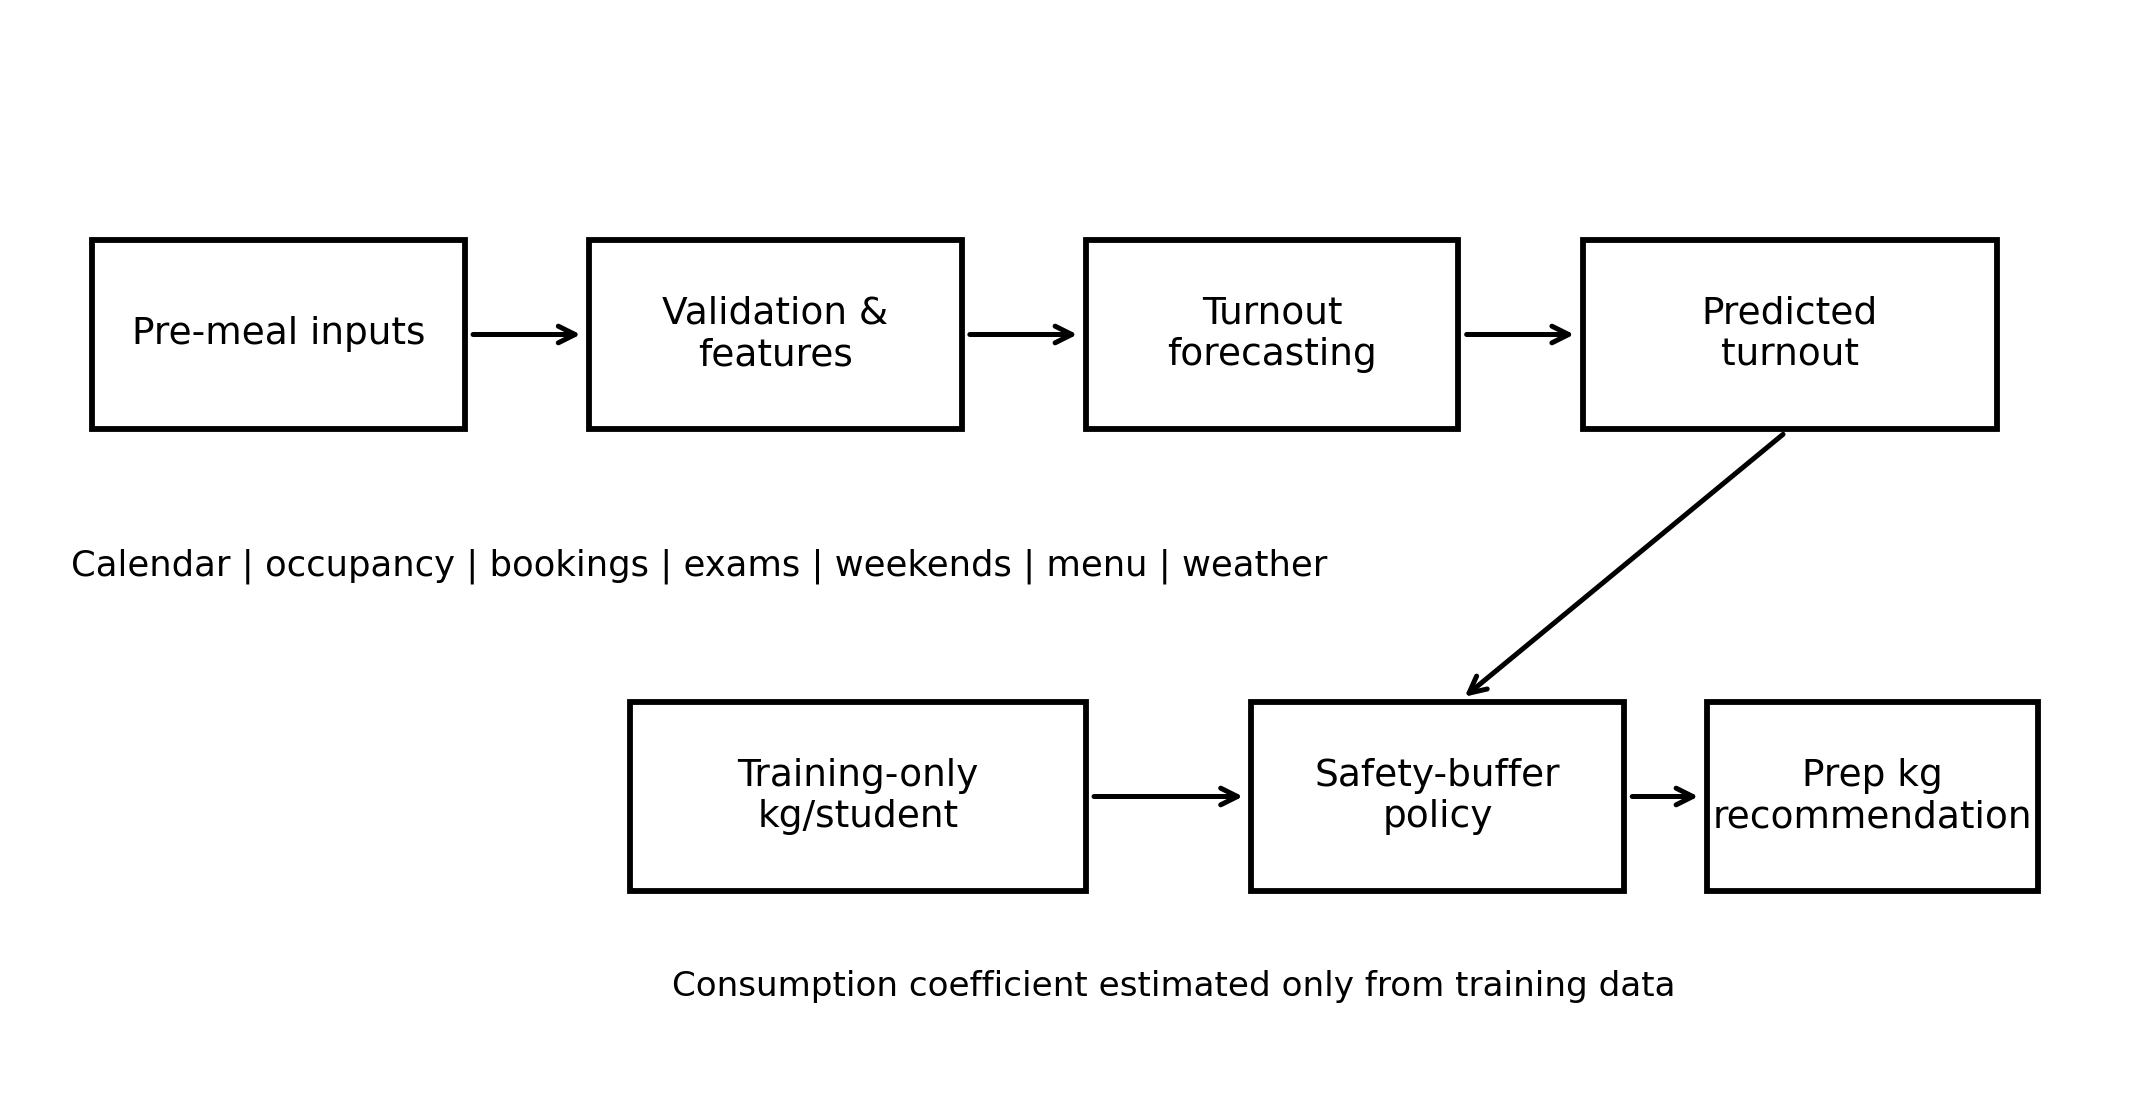
\includegraphics[width=0.95\columnwidth]{figures/system_architecture.png}
\caption{End-to-end system architecture.}\label{fig:architecture}
\end{figure}

\subsection{Experimental Results}\label{experimental-results}

\subsubsection{Forecasting Performance}\label{forecasting-performance}

Table I reports results for the chronological holdout.

\textbf{TABLE I. TURNOUT FORECASTING PERFORMANCE ON SYNTHETIC HOLDOUT
DATA}

\begin{center}
\resizebox{0.98\columnwidth}{!}{%
\begin{tabular}{@{}lrrr@{}}
\toprule\noalign{}
Model & MAE (students) & RMSE (students) & R² \\
\midrule\noalign{}
\bottomrule\noalign{}
Linear Regression & 10.158 & \textbf{12.825} & \textbf{0.9736} \\
XGBoost & \textbf{10.345} & 13.152 & 0.9722 \\
Random Forest & 10.565 & 13.521 & 0.9706 \\
\end{tabular}%
}
\end{center}

The three methods perform similarly, with R² values above 0.97. XGBoost
obtains the lowest MAE, while Linear Regression obtains the lowest RMSE
and highest R². Under the repository's model-selection rule, the Linear
Regression pipeline is therefore serialized as the best model.

\begin{figure}
\centering
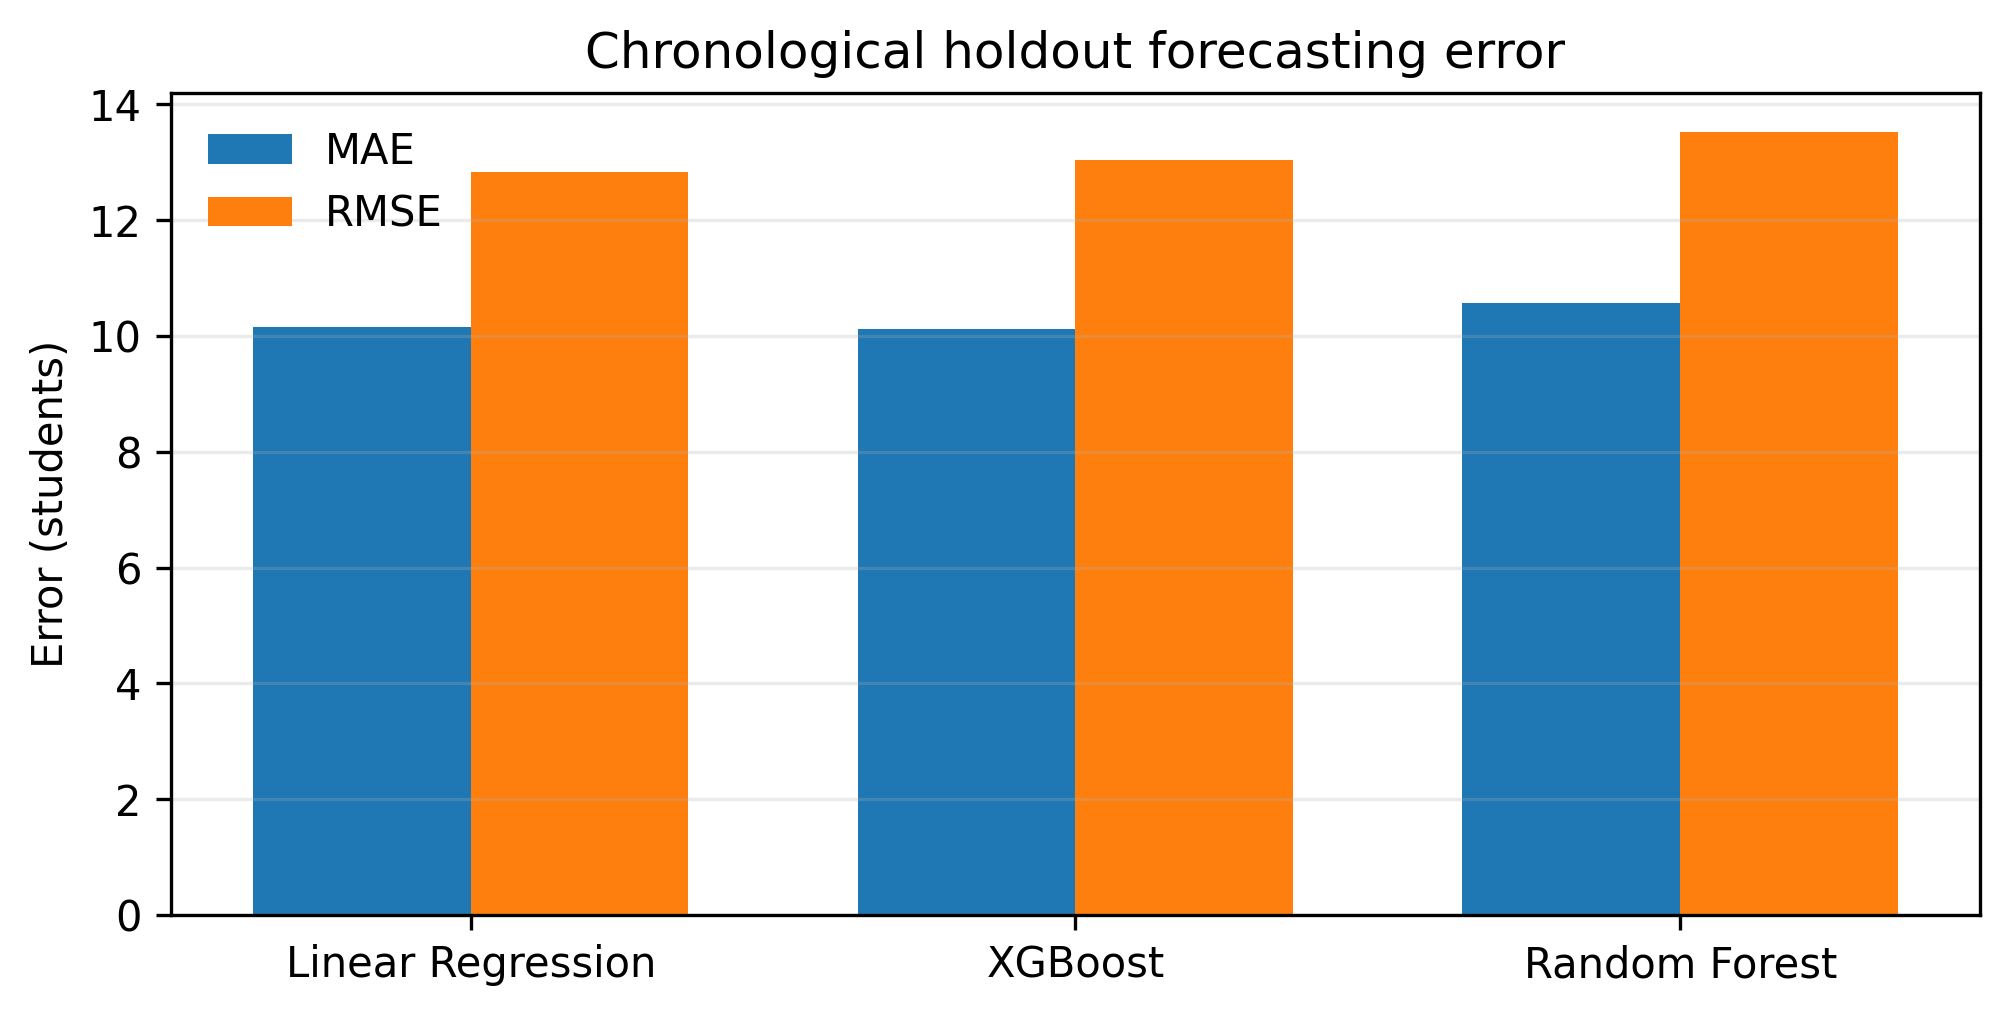
\includegraphics[width=0.95\columnwidth]{figures/model_error_comparison.png}
\caption{MAE and RMSE comparison across the three turnout models on the
chronological synthetic holdout.}\label{fig:modelerrors}
\end{figure}

This result is informative rather than problematic. The synthetic
generator contains strong structured relationships among residents
present, bookings, meal category, and turnout. Although nonlinearities
and interactions are included, the resulting data-generating process
remains sufficiently regular that a linear model can approximate it
well. In a real hostel, attendance behavior may contain more abrupt
nonlinearities, cohort effects, menu-specific preferences,
academic-event interactions, and drift, potentially changing the model
ranking. The inclusion of Random Forest and XGBoost in the package is
therefore valuable even though they do not dominate the default
synthetic run.

MAE and RMSE should also be interpreted in operational terms. An MAE of
approximately ten students means that the forecast is typically wrong by
about ten attendees per meal in the synthetic holdout. For a lunch
consumption coefficient near 0.54 kg per attending student, such an
error corresponds to roughly 5.4 kg before applying a safety buffer.
This direct relationship between forecast error and kilograms motivates
the second-stage preparation policy.

\subsubsection{Consumption Coefficients}\label{consumption-coefficients}

Training data produced the median per-student consumption coefficients
shown in Table II.

\textbf{TABLE II. TRAINING-SET MEDIAN CONSUMPTION PER ATTENDING STUDENT}

\begin{center}
\resizebox{0.98\columnwidth}{!}{%
\begin{tabular}{@{}lr@{}}
\toprule\noalign{}
Meal & Median kg/student \\
\midrule\noalign{}
\bottomrule\noalign{}
Breakfast & 0.3599 \\
Lunch & 0.5393 \\
Dinner & 0.4904 \\
\end{tabular}%
}
\end{center}

These coefficients are estimated only from training observations,
preventing test-set outcomes from influencing the recommendation
formula.

\subsubsection{Operational Simulation}\label{operational-simulation}

Using the best-RMSE forecast model and a 3\% safety buffer, recommended
preparation is calculated for each holdout meal. Table III summarizes
the results.

\textbf{TABLE III. RETROSPECTIVE PREPARATION-POLICY SIMULATION}

\begin{center}
\resizebox{0.98\columnwidth}{!}{%
\begin{tabular}{@{}lr@{}}
\toprule\noalign{}
Metric & Value \\
\midrule\noalign{}
\bottomrule\noalign{}
Actual synthetic food prepared & 76,234.07 kg \\
Recommended preparation & 71,418.43 kg \\
Change in preparation & -6.317\% \\
Recorded synthetic waste & 8,423.00 kg \\
Simulated leftover under recommendation & 2,600.69 kg \\
Simulated leftover reduction & 69.124\% \\
Simulated shortage & 749.03 kg \\
Shortage / realized consumption & 1.077\% \\
\end{tabular}%
}
\end{center}

The simulation suggests that forecast-guided preparation can
substantially reduce modeled leftovers, but it also demonstrates why
waste reduction cannot be evaluated without shortage. If the system
minimized preparation mass alone, waste could be driven down by
systematically under-serving students. The explicit shortage metric
reveals this failure mode.

The default 3\% buffer yields simulated shortages equal to 1.077\% of
realized food consumption over the holdout. A production deployment
should calibrate this parameter with institutional policy. For example,
a hostel may prefer a larger buffer during lunch, examination periods,
or high-variability menus. More advanced extensions could predict
conditional quantiles rather than a single expected turnout and select
preparation from a desired service percentile.

\begin{figure}
\centering
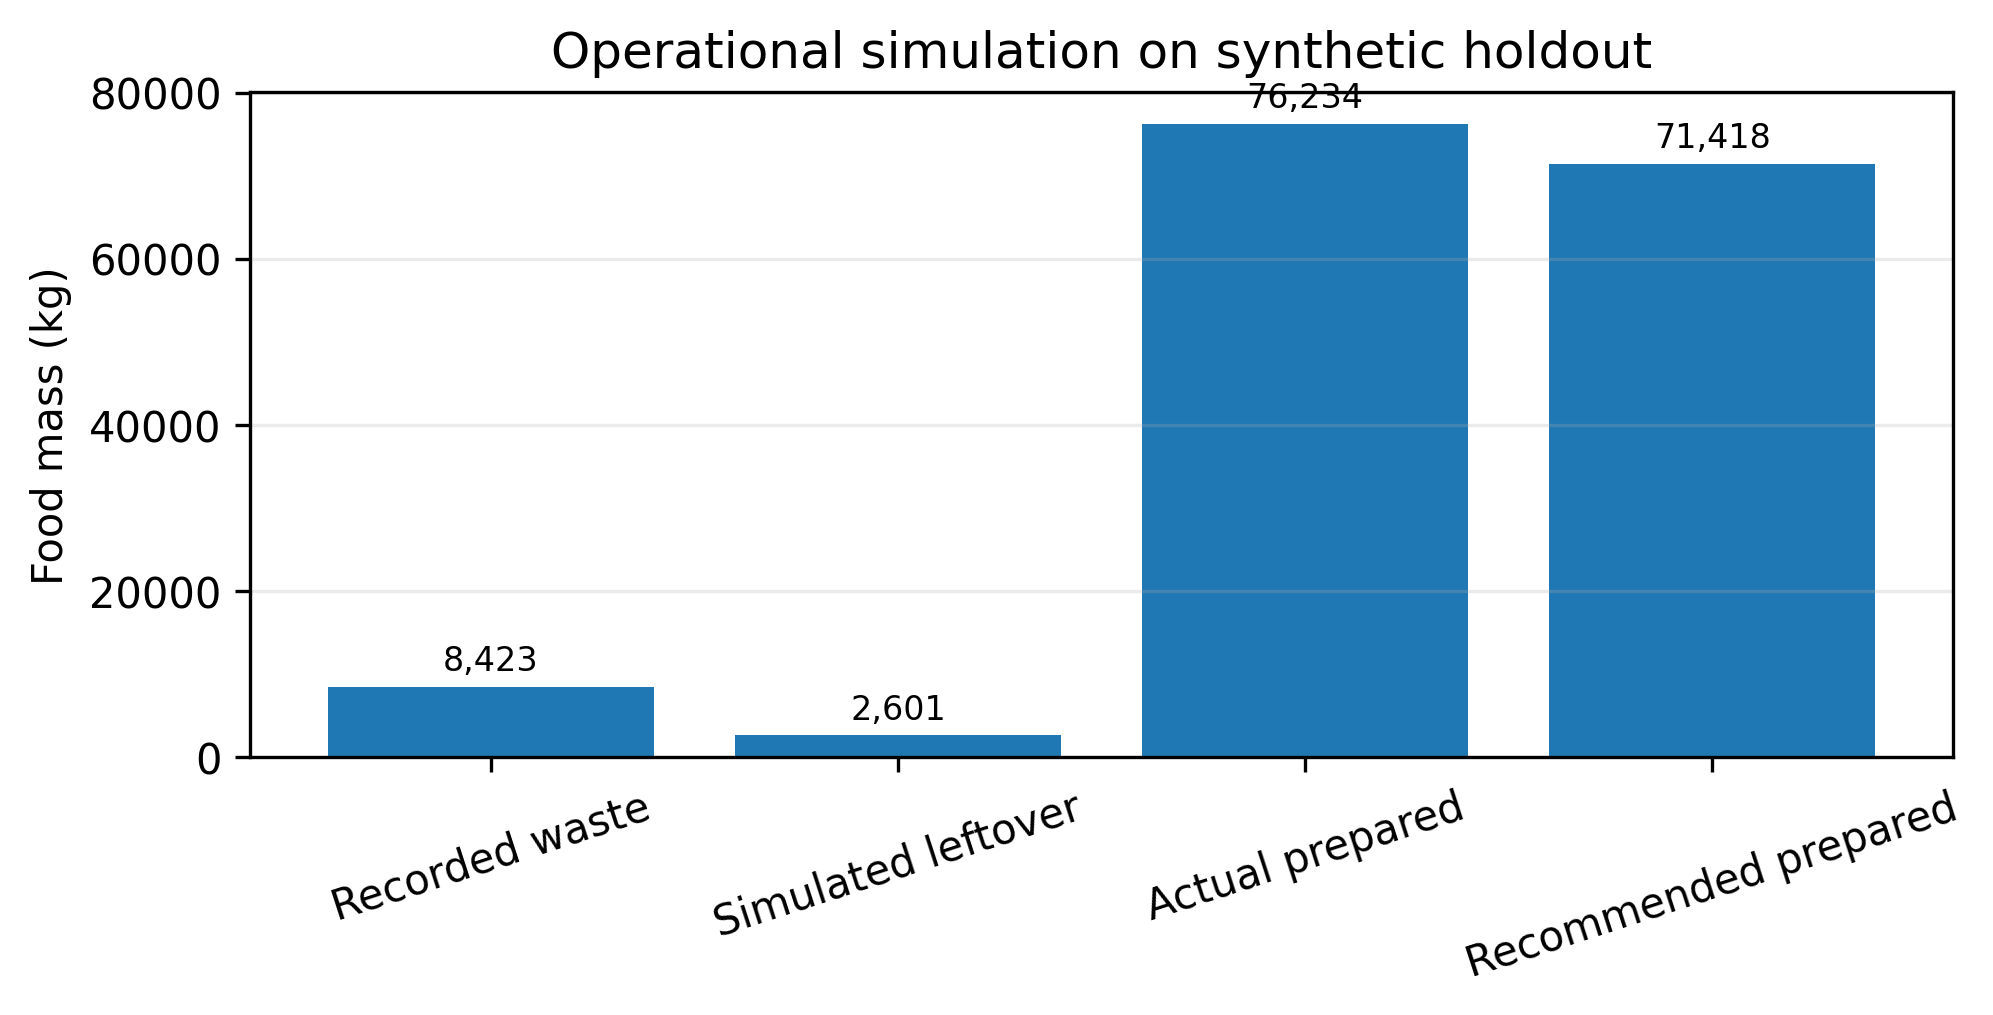
\includegraphics[width=0.95\columnwidth]{figures/operational_simulation.png}
\caption{Comparison of recorded synthetic waste/actual preparation and
forecast-guided simulated leftovers/recommended
preparation.}\label{fig:ops}
\end{figure}

\subsubsection{Comparison with Prior
Work}\label{comparison-with-prior-work}

The direction of the simulation is consistent with prior literature
arguing that improved demand estimates can reduce overproduction in
catering {[}3{]}, {[}7{]}. However, the magnitude of the 69.124\%
simulated leftover reduction must \textbf{not} be compared directly with
empirical reductions reported by other studies. The current figure is
generated under a synthetic data-generating process in which actual
preparation is intentionally conservative. It demonstrates how the
decision policy behaves under controlled assumptions, not how much waste
a real institution would save.

\subsubsection{Reproducibility}\label{reproducibility}

The repository fixes random seeds, saves the generated dataset, stores
full row-level holdout predictions, records model metadata, and exposes
all hyperparameters in source code. The complete experiment can be
reproduced with two commands: one to generate data and one to
train/evaluate models. Unit tests validate minimum dataset size and
recommendation bounds. These features make the package suitable for
interview demonstration, capstone assessment, and extension to real
records.

\subsection{Discussion}\label{discussion}

\subsubsection{Why Forecasting and Recommendation Are
Separated}\label{why-forecasting-and-recommendation-are-separated}

A key architectural choice is not to train a model that directly
predicts ``food to prepare'' using historical prepared-food values.
Historical preparation is itself a human decision and can encode past
overproduction practices. A model trained to imitate it may reproduce
waste rather than reduce it. The proposed architecture predicts turnout,
estimates consumption, and then applies an explicit policy. This makes
the decision logic observable and tunable.

The same separation also supports governance. Kitchen managers can
adjust the safety buffer without retraining the demand model. They can
review meal-specific consumption coefficients and compare predictions
with bookings. If an institution decides that shortage is five times
more costly than leftover food, the policy layer can reflect that
operational preference.

\subsubsection{Feature Availability and
Deployment}\label{feature-availability-and-deployment}

The current features are plausible for a digital hostel environment.
Residents present can be estimated from occupancy/leave systems; advance
bookings can come from a meal-booking portal; exam and vacation flags
can come from an academic calendar; menu information comes from kitchen
planning; and weather can be obtained through external APIs. A real
deployment should record the timestamp at which each feature becomes
available to ensure that training faithfully represents inference-time
conditions.

\subsubsection{Model Monitoring}\label{model-monitoring}

Deployment creates several monitoring requirements. Prediction error
should be tracked by meal category, day type, exam status, and menu.
Data drift can be detected when distributions of bookings, occupancy, or
menu categories move away from the training baseline. Operational
monitoring should track both leftover kilograms and shortage events. A
low model RMSE is insufficient if systematic under-preparation occurs
for a subgroup of meals.

\subsubsection{Privacy and Data
Minimization}\label{privacy-and-data-minimization}

The proposed model does not require personally identifiable student
attributes. Aggregate counts---residents present and advance
bookings---are sufficient for the baseline architecture. This is
preferable for privacy and simplifies governance. If future research
introduces cohort, dietary, or demographic variables, institutional
approval, minimization, access control, and fairness analysis should be
considered.

\subsubsection{Limitations}\label{limitations}

The most important limitation is the synthetic nature of the current
dataset. The generator encodes assumed relationships, and models trained
on those relationships may recover the generator rather than discover
unknown behavior. High R² values therefore demonstrate software and
modeling consistency, not field generalization.

Second, the operational simulation assumes that consumed kilograms are
an appropriate demand proxy and that preparation can be scaled
proportionally by attendance. Real kitchens prepare menu items in
batches and may face minimum batch sizes, ingredient constraints, recipe
yields, dietary categories, and uncertain plate waste. Third, the model
treats meals as tabular observations rather than explicitly modeling
temporal autocorrelation across consecutive days. Lag features,
hierarchical time-series methods, probabilistic forecasting, and
recurrent or transformer models may improve performance when longer real
datasets are available.

Fourth, the recommendation uses a fixed 3\% buffer. A constant buffer is
transparent but may be suboptimal. Risk-aware quantile regression could
directly estimate an upper attendance percentile, and constrained
optimization could choose item-level production quantities based on
shortage cost, waste cost, and batch constraints.

\subsection{Deployment Roadmap}\label{deployment-roadmap}

A practical institutional rollout can be staged.

\textbf{Phase 1---Observation:} collect at least one academic year of
audited meal-level data, including attendance, prepared quantity,
leftover quantity, bookings, menu, academic calendar, and occupancy.
Establish measurement definitions before model fitting.

\textbf{Phase 2---Shadow forecasting:} run the model without influencing
kitchen decisions. Compare predicted turnout with actual turnout and
quantify errors by meal and calendar condition.

\textbf{Phase 3---Advisory mode:} show predicted turnout and recommended
preparation to kitchen staff while retaining human approval. Record
whether staff accept or modify each recommendation.

\textbf{Phase 4---Controlled intervention:} conduct an A/B or
stepped-wedge operational study across comparable meal periods,
measuring waste, shortage, cost, and student-service outcomes.

\textbf{Phase 5---Continuous learning:} retrain on newly audited
observations, monitor drift, recalibrate safety buffers, and integrate
item-level demand if data quality supports it.

This staged approach turns the current capstone from a model
demonstration into a testable socio-technical intervention.

\subsection{Conclusion}\label{conclusion}

This paper presented an end-to-end AI-driven framework for hostel
food-waste mitigation through demand forecasting and explicit
preparation control. The system combines a reproducible synthetic data
generator, leakage-aware features, chronological validation, Linear
Regression, Random Forest, and XGBoost turnout models, and a
meal-specific kilogram recommendation policy. On 441 chronological
synthetic holdout observations, all three models achieved R² above 0.97;
Linear Regression obtained the best RMSE at 12.825 students while
XGBoost obtained the best MAE at 10.345 students. A 3\% safety-buffer
simulation reduced modeled leftovers while retaining a separately
quantified shortage rate.

The primary contribution is architectural: forecast demand using only
pre-meal variables, then convert the forecast to production through a
visible and tunable policy rather than learning directly from
potentially wasteful historical preparation. The implementation is fully
reproducible and can serve as an engineering capstone, interview
portfolio, or foundation for an institutional pilot. Future work should
replace synthetic data with audited hostel records, incorporate
probabilistic forecasting, optimize buffer levels under explicit
waste/shortage costs, and validate impact through prospective field
studies.

\subsection{References}\label{references}

{[}1{]} United Nations, ``Goal 12: Ensure sustainable consumption and
production patterns,'' Sustainable Development Goals, Target 12.3.
{[}Online{]}. Available: https://sdgs.un.org/goals/goal12

{[}2{]} United Nations Environment Programme, \emph{Food Waste Index
Report 2024}. Nairobi, Kenya: UNEP, 2024.

{[}3{]} M. Rodrigues, V. Miguéis, S. Freitas, and T. Machado, ``Machine
learning models for short-term demand forecasting in food catering
services: A solution to reduce food waste,'' \emph{Journal of Cleaner
Production}, vol.~435, Art. no. 140265, 2024, doi:
10.1016/j.jclepro.2023.140265.

{[}4{]} M. Faezirad, A. Pooya, Z. Naji-Azimi, and M. Amir Haeri,
``Preventing food waste in subsidy-based university dining systems: An
artificial neural network-aided model under uncertainty,'' \emph{Waste
Management \& Research}, vol.~39, no. 8, pp.~1027--1038, 2021, doi:
10.1177/0734242X211017974.

{[}5{]} G. F. Turker, ``Reducing food waste in campus dining: A
data-driven approach to demand prediction and sustainability,''
\emph{Sustainability}, vol.~17, no. 2, Art. no. 379, 2025, doi:
10.3390/su17020379.

{[}6{]} B. Aydın, Y. S. Balcıoğlu, and B. Sezen, ``Machine learning
techniques for cafeteria demand forecasting: An institutional case,''
\emph{OPUS Journal of Society Research}, vol.~22, no. 3, pp.~532--549,
2025, doi: 10.26466/opusjsr.1649256.

{[}7{]} C. Malefors, L. Secondi, S. Marchetti, and M. Eriksson, ``Food
waste reduction and economic savings in times of crisis: The potential
of machine learning methods to plan guest attendance in Swedish public
catering during the Covid-19 pandemic,'' \emph{Socio-Economic Planning
Sciences}, vol.~82, Art. no. 101041, 2022, doi:
10.1016/j.seps.2021.101041.

{[}8{]} A. Dhir, S. Talwar, P. Kaur, and A. Malibari, ``Food waste in
hospitality and food services: A systematic literature review and
framework development approach,'' \emph{Journal of Cleaner Production},
vol.~270, Art. no. 122861, 2020, doi: 10.1016/j.jclepro.2020.122861.

{[}9{]} K. Posch, C. Truden, P. Hungerländer, and J. Pilz, ``A Bayesian
approach for predicting food and beverage sales in staff canteens and
restaurants,'' \emph{International Journal of Forecasting}, vol.~38, no.
1, pp.~321--338, 2022, doi: 10.1016/j.ijforecast.2021.06.001.

{[}10{]} Y. Li, C. Zhang, H. Xu, Y. Yang, H. Lu, and L. Deng,
``Strategies for automated identification of food waste in university
cafeterias: A machine vision recognition approach,'' \emph{Applied
Sciences}, vol.~15, no. 9, Art. no. 5036, 2025, doi:
10.3390/app15095036.

{[}11{]} Y. Kim and H. S. Yoon, ``Leveraging machine learning to predict
food waste quantity: Focusing on military dining facilities as
large-scale food service operations,'' \emph{Journal of Forecasting},
vol.~45, no. 4, pp.~2001--2016, 2026, doi: 10.1002/for.70128.

{[}12{]} L. Breiman, ``Random forests,'' \emph{Machine Learning},
vol.~45, pp.~5--32, 2001, doi: 10.1023/A:1010933404324.

{[}13{]} T. Chen and C. Guestrin, ``XGBoost: A scalable tree boosting
system,'' in \emph{Proc. 22nd ACM SIGKDD Int. Conf. Knowledge Discovery
and Data Mining}, 2016, pp.~785--794, doi: 10.1145/2939672.2939785.

{[}14{]} F. Pedregosa \emph{et al.}, ``Scikit-learn: Machine learning in
Python,'' \emph{Journal of Machine Learning Research}, vol.~12,
pp.~2825--2830, 2011.

\begin{center}\rule{0.5\linewidth}{0.5pt}\end{center}
\end{document}
